% !TeX encoding = UTF-8
% !TeX program = pdflatex
% !TeX spellcheck = it_IT

\documentclass[binding=0.6cm, a4paper]{unifith/unifith}
\usepackage{microtype}
\usepackage[english]{babel}
\usepackage[utf8]{inputenc}
\usepackage{amssymb}
\usepackage{mathtools,amsmath}
\usepackage{slashed}
\usepackage{physics}
\usepackage{breqn}
\usepackage{afterpage}
\usepackage{appendix}
\usepackage{cancel}
\usepackage{comment}
\usepackage[dvipsnames]{xcolor}
\usepackage{listings}
\usepackage{hyperref}
\usepackage{graphicx}
\usepackage{mathbbol}
\usepackage{amssymb}
\usepackage{amsthm}
\usepackage{soul}
\usepackage{empheq}
\usepackage[framed,numbered,autolinebreaks,useliterate]{unifith/mcode}
\theoremstyle{plain}
\newtheorem{thm}{Theorem}[chapter]
\theoremstyle{definition}
\newtheorem{defn}[thm]{Definition}
\newtheorem{exmp}[thm]{Example}
\DeclareSymbolFontAlphabet{\amsmathbb}{AMSb}%
\graphicspath{}

% Remove in a normal thesis
\newcommand{\bs}{\textbackslash}
\newcommand{\be}{\begin{equation}}
\newcommand{\ee}{\end{equation}}
\newcommand{\bee}{\begin{equation*}}
\newcommand{\eee}{\end{equation*}}
\newcommand{\mn}{\mu\nu}
\newcommand{\ty}{\tilde{y}}
\newcommand{\tx}{\tilde{x}}
\newcommand{\csb}{$\chi$SSB}
\newcommand{\deq}{\vcentcolon=}
\newcommand{\eqd}{=\vcentcolon}

\begin{document}

\lstset{language=Matlab,%
    breaklines=true,%
    morekeywords={matlab2tikz},
    keywordstyle=\color{blue},%
    morekeywords=[2]{1}, keywordstyle=[2]{\color{Black}},
    identifierstyle=\color{Black},%
    stringstyle=\color{VioletRed},
    commentstyle=\color{Green},%
    showstringspaces=false,%without this there will be a symbol in the places where there is a space
    numbers=left,%
    numberstyle={\tiny \color{Black}},% size of the numbers
    numbersep=4pt, % this defines how far the numbers are from the text
}


\chapter*{Action optimization using The Surface Evolver}

The physical problem (just for context) is to calculate the rate of a phase transition for a particular theory. The same phenomenon that interests the boiling water(nucleation and expansion of bubble, change of state), also happens in the theory I am considering. To find the observable value $\Gamma$, i.e. the rate at which the bubbles form, I must know the value of the \textbf{"action" function} $S$ of my theory, evaluated on a configuration that \textbf{makes it stationary}. We have reasons to believe that this configuration is neither a minimum nor a maximum of the action, but instead, it is a \textbf{saddle point} of it; it is called a "bounce solution", it will have subscript "b".

\section*{WSS action}

The functional action to which I refer is the Witten-Sakai-Sugimoto (WSS) action: 
\begin{equation}
    S[z(x,y)]\deq \int \dd x\dd y x^2 y^{5/2} \sqrt{1+\left(y^3-1\right) \left(\partial_y z\right)^2+\left(\partial_x z\right)^2}.\label{Stilde}
\end{equation}
This is the general formula for this action: it is a 2-dimensional integral over the domain of both $x$ and $y$, a function of the surface $z(x,y)$. After a rewriting, specifying the domain of integration, the action evaluated on $z(x,y)=z_b(x,y)$ which is the configuration that makes it stationary takes the form

\begin{multline}\label{DELTASTILDE}
S=2\int_0^\infty \dd x \int_{y_J(x)}^\infty\dd y \sigma^2 y^{5/2}\left( \sqrt{1+\left(y^3-1\right) \left(\partial_y z_b\right)^2+\left(\partial_x z_b\right)^2}-1\right)\\
-2\int_0^\infty \dd x \int_1^{y_J(x)}\dd y x^2 y^{5/2}
\end{multline}

It is clear that the integration domain is nontrivial: the curve $y_J(x)$ is a curve with endpoints on the $x$ and $y$ axes, and it is entirely in the $(x,y)$ plane.

The curve $y_J(x)$ is not fixed, and thus must be dynamically determined by extremizing \eqref{DELTASTILDE} as we will do for $z_b(x,y)$: the state space of the complete variational problem is, therefore, a Cartesian product between all possible curves $y(x)$ and all possible surfaces $z(x,y)$ with the appropriate domain and boundary conditions, and the aim is to find the correct $y_J(x)$ and $z_b(x,y)$ that extremize $S$. Every time I write $S$ I will actually mean $S[z_b(x,y),y_J(x)]$. 

Now, if the boundary curve of the integration domain $y_J(x)$ is fixed, it can be shown that the problem is of strictly convex nature: therefore, the \textit{fixed boundary problem} of finding $z_b$ is a \textit{minimum} problem, while the free boundary problem of finding $[z_b,y_J]$ is a \textit{saddle point} problem. I have already solved the fixed boundary case using MATLAB, but the free boundary case is a lot more complex.

To make the formulas usable for numerical work, I rewrote \eqref{DELTASTILDE}: first performing a compactification of the integration variables, so that the domain is entirely in the unit square, using
\begin{align}
    \tilde{x}&=\frac{2}{\pi}\arctan(x),\\
    \tilde{y}&=\frac{2}{\pi}\arctan(y-1), 
\end{align}
and the integral will become
\begin{multline}
    S=2\pi^2\int_0^1 \dd \tilde{x} \int_{\tilde{y}_J(\tilde{x})}^1\dd \ty f_3(\tilde{x}) f_4(\ty)\left( \sqrt{1+f_1(\ty) \left(\partial_\ty z_b\right)^2+f_2(z)\left( \partial_{\tilde{x}} z_b\right)^2}-1\right)\\
    -2\pi^2\int_0^1 \dd \tilde{x} \int_0^{\tilde{y}_J(z)}\dd \ty f_3(\tilde{x}) f_4(\ty),
\end{multline}
where
\begin{align*}
    \ty_J(\tx)&=\frac{2}{\pi}\arctan(y_J(x(\tx))-1);\\
    f_1(\ty)&=\frac{1}{\pi^2}\left(\sin(\pi\ty)(4+3\sin(\pi\ty))+\sin(2\pi\ty)\right);\\
    f_2(\tx)&=\frac{4}{\pi^2}\cos^4\left(\frac{\pi \tx}{2}\right);\\
    f_3(\tx)&=\frac{\tan^2\left(\frac{\pi \tx}{2}\right)}{1+\cos(\pi \tx)};\\
    f_4(\ty)&=\frac{\left(\tan\left(\frac{\pi \ty}{2}\right)+1\right)^{5/2}}{1+\cos(\pi \ty)}.
\end{align*}
It is important to point out that the curve $\ty_J$, up to here described as a function $\ty_J(\tx)$, might generally not be univalent and therefore need a parametric curve description. We will still call it $\ty_J$ for simplicity, but I will mean a curve with parametric coordinate $t$ and equation 
\begin{equation}
    \{\tx_J(t),\ty_J(t)\}:[0,1]\rightarrow\left([0,1]\cross[0,1]\right),\quad \tx_J(0)=0,\;\ty_J(1)=0,
\end{equation}
i.e. starts on the $y$ axis and ends on the $x$ axis.
Finally, I write 
\begin{empheq}[box=\fbox]{multline}\label{numericaldbiaction}
    S=2\pi^2\int_{\Omega[\ty_J]} \dd A \;f_3(\tx)f_4(\ty)\left( \sqrt{1+f_1(\ty) \left(\partial_\ty z_b\right)^2+f_2(\tx)\left(\partial_\tx z_b\right)^2}-1\right)\\
    -2\pi^2\int_{\Xi[\ty_J]} \dd A \;f_3(\tx) f_4(\ty),
\end{empheq}
where $\dd A=\dd A(\tx,\ty)$ is the area element, and the integrals are performed on the complementary domains $\Omega[\ty_J]$ and $\Xi[\ty_J]$, together forming a unit square $[0,1]\cross[0,1]$, separated by the curve $\ty_J$. The $\Omega[\ty_J]$ part is defined as the one containing the point $(1,1)$, while the $\Xi[\ty_J]$ part contains the point $(0,0)$.

The boundary conditions for the bounce $z_b$ are:
\begin{equation}\label{bouncedbiconditions}
    \begin{dcases}
        \lim_{\tx\rightarrow 1}z_b(\tx,\ty)=L\\
        \lim_{\ty\rightarrow 1}z_b(\tx,\ty)=L\\
        \eval{\partial_\tx z_b(\tx,\ty)}_{\tx=0}=0
    \end{dcases}
\end{equation}

\subsection*{Figures}

Here are some examples that I think can show the nature of the problem, regarding both the surface and the domain of integration.



\begin{figure}[htbp]
    \centering
    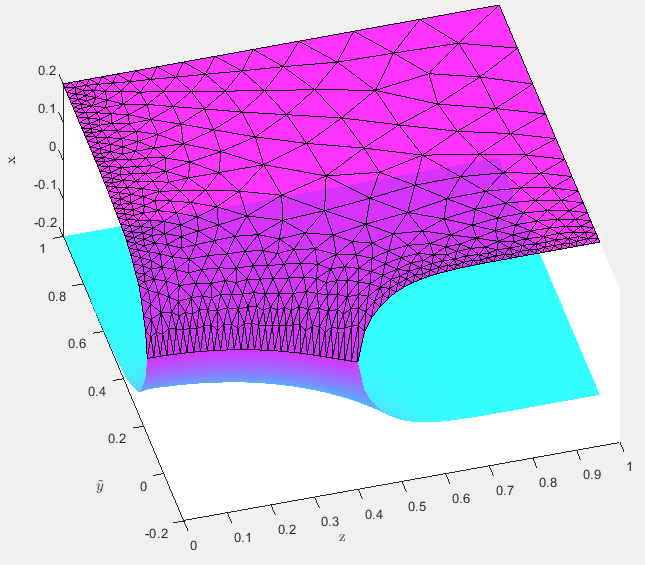
\includegraphics[scale=.55]{images/waffle.png}
    \caption{An example of a possible bounce solution to show its boundary conditions. The surface was obtained by a minimization of the action, but the domain boundary curve $\ty_J(\tx)$ was guessed. For physical reasons, here is also drawn a mirrored image (in light blue), but the calculation was only done on the purple simplicial complex. Also, please notice that in the picture the labels "x" and "z" are switched.}
    \label{fig:bounceexample}
\end{figure}

\begin{figure}[htbp]
\centering
    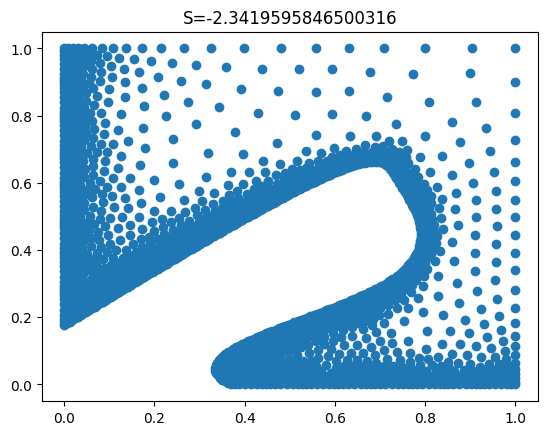
\includegraphics[width=.4\textwidth]{images/download.png}
\qquad
    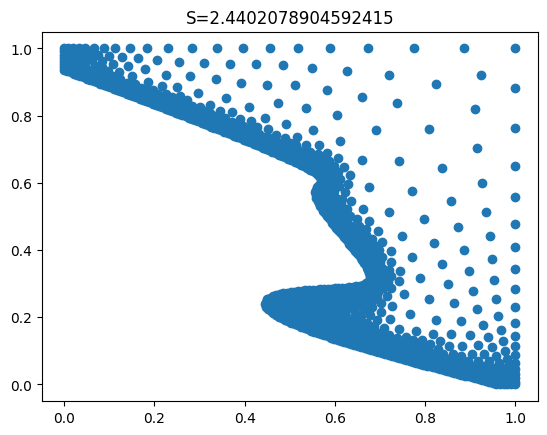
\includegraphics[width=.4\textwidth]{images/trasferimento (1).png}
\qquad
    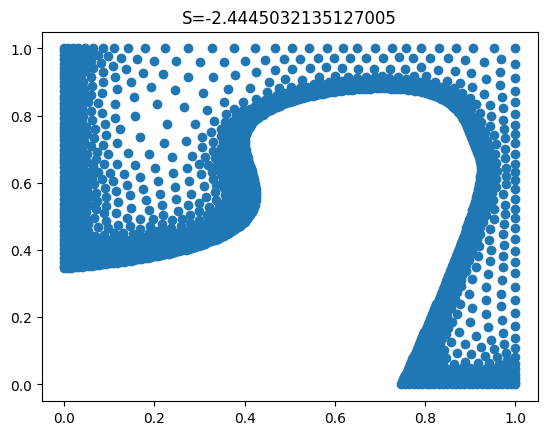
\includegraphics[width=.4\textwidth]{images/trasferimento (2).png}
\qquad
    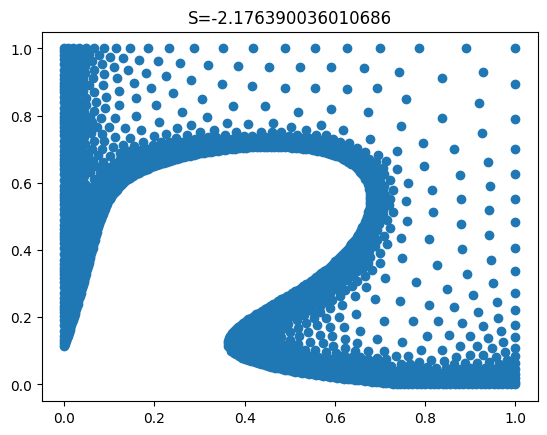
\includegraphics[width=.4\textwidth]{images/trasferimento (3).png}
\qquad
    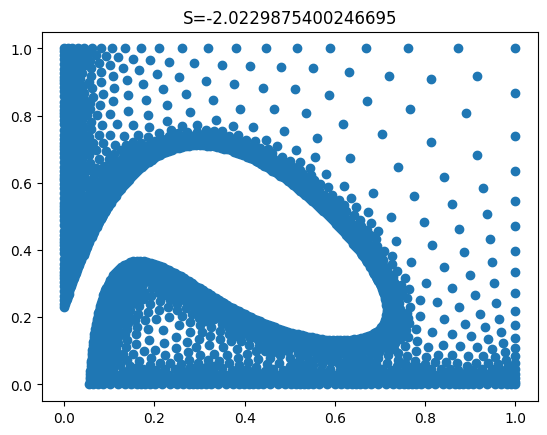
\includegraphics[width=.4\textwidth]{images/trasferimento.png}
    \qquad
    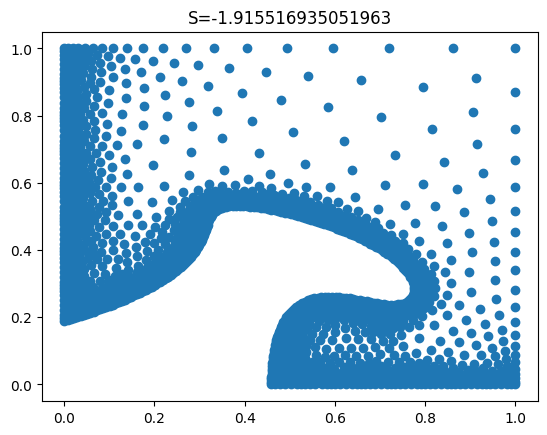
\includegraphics[width=.4\textwidth]{images/trasferimento (4).png}
\caption{Examples of the possible integration domains. It is \textit{expected} a simple domain like the one used in figure \ref{fig:bounceexample}, but in principle any curve is good. The colored region is $\Omega[\ty_J]$, and the white one is $\Xi[\ty_J]$. On top of each is the value of the action evaluated on the "fixed-domain-bounce".\label{fig:i}}
\end{figure}

\section*{Implementation with The Surface Evolver}

I tried to solve this problem with The Surface Evolver, but I couldn't figure out how. I defined the action (splitting it into two pieces, "action" and "falseaction", the first is integrated on $\Omega[\ty_J]$ and the latter on $\Xi[\ty_J]$). I defined the geometry using vertices, edges, and faces, and the boundary conditions were informed via the three simple constraints. The thing I see when opening the program is promising, but I can't understand if the simulation is converging. If I try to set a greater modulus for the actions, the simulation just blows up.

In the definitions, $L$ is the same as in \eqref{bouncedbiconditions}, $qq$ is put there instead of $1$ so that the tangents don't diverge, and $rx,ry$ are just starting points for the boundary curve.

I tried to implement the derivatives $\partial_\tx z$ and $\partial_\ty z$ as ratios of the components of the normal vector (hoping I understood correctly the meaning of $x4,x5,x6$).

I mentioned that the problem will be a saddle-point problem, thus minimizing the action won't solve it, but I thought that it was sensible to first understand the software with a simple minimization problem, and then move to the more complex saddle-point.


\end{document}